
\documentclass{report}

\chapter{Pygmalion-Like-Reimplementation User Documentation}

\section{Running the program}
To compile and run the software, you need to have \texttt{dotnet} and \texttt{npm} available on your system.
The required .NET Runtime version is 8.X.

Compilation can be done using these commands (run in the root directory of the project):
\begin{Verbatim}
dotnet tool install fable
dotnet tool restore
dotnet restore
npm update
npm run build
\end{Verbatim}

The webpage is then available in the \texttt{dist} directory. It can be run by using the command:
\begin{Verbatim}
npm run server
\end{Verbatim}
This will open a local HTTP server on \url{http://127.0.0.1:5173/} which hosts the software.

\section{Using the software}

\begin{figure}[H]
    \centering
    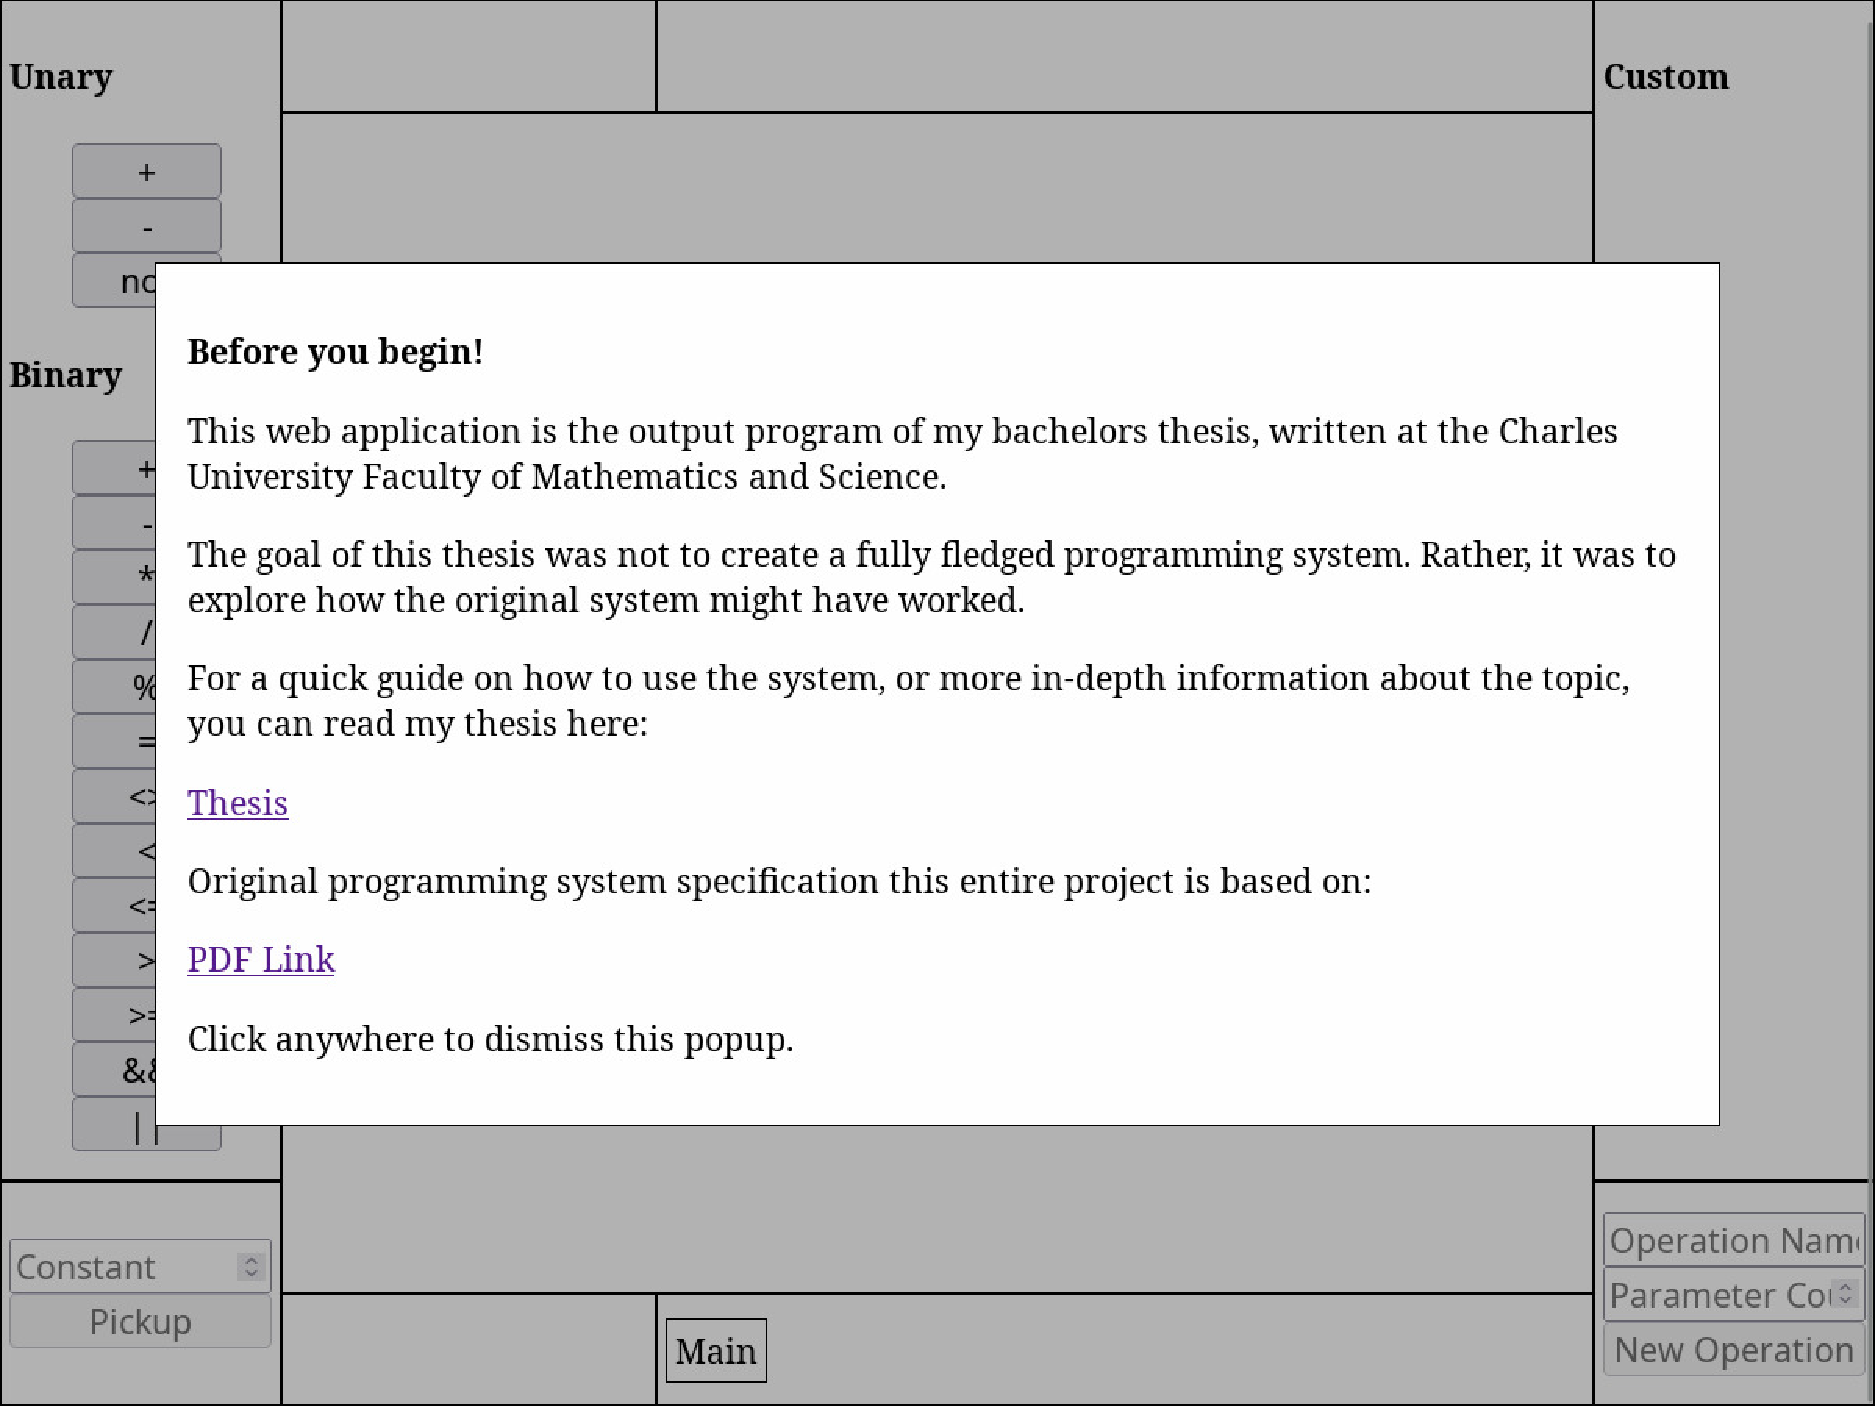
\includegraphics[width=0.8\textwidth]{img/app_intro.pdf}
    \caption{The first screen the user sees}
    \label{fig:intro}
\end{figure}

The software is a web application that can be accessed through a web browser. The first thing the user sees is an intro popup. It can be dismissed by clicking anywhere on the screen.

\begin{figure}[H]
    \centering
    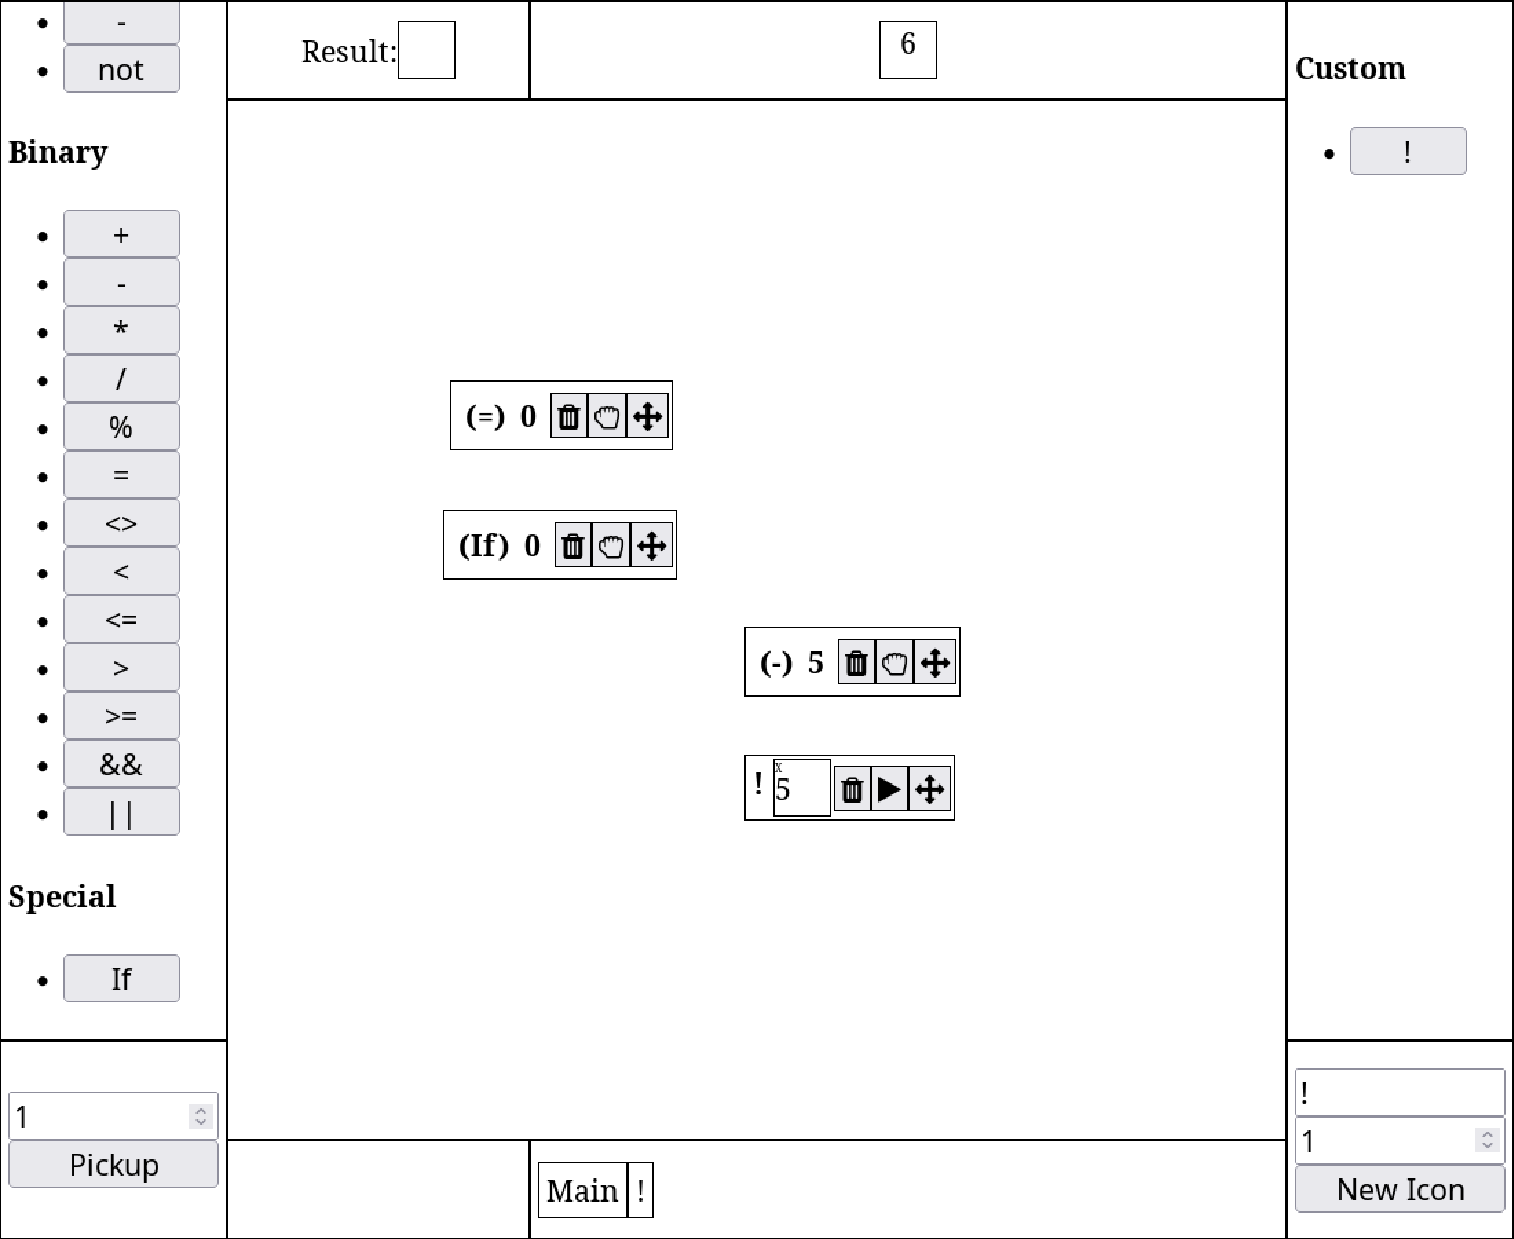
\includegraphics[width=0.8\textwidth]{img/app.pdf}
    \caption{The GUI of the software}
    \label{fig:gui}
\end{figure}

The GUI is split into nine parts. The split can be seen in Figure \ref{fig:gui}.
